% Este archivo no es definitivo. Solo cuenta con el material que 
% me pareció más importante y que debo estudiar. 
% A falta de tiempo, solo dejaré lo más importante en cada caso.

\section{Dinámica de los instrumentos indicadores}

Un instrumento analógico se compone de dos partes: una fija (estator) y una móvil (rotor). 
El principio es físico es simple: una fuerza (dependiente de la magnitud eléctrica a medir) empuja al rotor, produciendo un giro. A la relación entre lo que medimos y cuánto gira la aguja se le llama \emph{ley del instrumento}.

Resumen de los principales tipos de instrumentos y sus leyes de respuesta:

\begin{description}
  \item \textbf{Imán permanente y bobina móvil (PMMC)}
    \begin{itemize}
      \item \textit{Mide:} Corriente y tensión en \textbf{C.C.}
      \item \textit{Ley:} Lineal (\(\alpha = K \cdot i\)).
    \end{itemize}
  \item \textbf{Hierro móvil}
    \begin{itemize}
      \item \textit{Mide:} Corriente y tensión en \textbf{C.C. y C.A.}
      \item \textit{Ley:} Cuadrática (\(\alpha = \frac{dL}{d\alpha}I^2\)).
    \end{itemize}
  \item \textbf{Electrodinámico}
    \begin{itemize}
      \item \textit{Mide:} Potencia, corriente, tensión.
      \item \textit{Ley:} Depende del coseno de fase (\(\alpha = \frac{dM}{d\alpha}I_fI_m \cos(\beta)\)).
    \end{itemize}
  \item \textbf{Inducción}
    \begin{itemize}
      \item \textit{Mide:} Energía (medidores de luz) y potencia en \textbf{C.A.}
      \item \textit{Ley:} Depende del seno (\(\alpha = K I_1 I_2 \sin(\beta)\)).
    \end{itemize}
\end{description}

\subsection{Ecuación general del movimiento (Las Cuplas)}

Para entender la dinámica, definiremos las fuerzas de rotación (Torques) como \textbf{Cuplas}. Para que la aguja se detenga en el valor correcto, deben interactuar tres tipos de cuplas:

\begin{enumerate}
    \item \textbf{Cupla Motora (\(C_m\)):} Es la fuerza que quiere mover la aguja. Su origen es eléctrico (magnético, electrostático, etc.).
    \item \textbf{Cupla Antagónica o Directriz (\(C_d\)):} Es la fuerza que ``tira hacia atrás''. Generalmente es un resorte que se retuerce. Si no existiera, la aguja daría vueltas completas como un motor.
    \item \textbf{Cupla de Amortiguamiento (\(C_a\)):} Es el freno. Solo aparece cuando hay movimiento y evita que la aguja oscile eternamente alrededor del valor final.
\end{enumerate}

La ecuación diferencial que describe el equilibrio dinámico es:
\[ C_m = C_d + C_a + C_i \]
Donde \(C_i\) es la inercia del sistema (\(J \frac{d^2\alpha}{dt^2}\)).

\subsection[Análisis de la Cupla Directriz]{Análisis de la Cupla Directriz (\(C_d\))}

La cupla directriz (o de restitución) suele generarse mediante resortes en espiral o cintas de torsión. Su fuerza es proporcional al ángulo girado (Ley de Hooke angular):
\[ C_d = K_r \cdot \alpha \]
Donde \(K_r\) depende del material (bronce-fosforoso) y la geometría del resorte.

\subsubsection{El proceso de equilibrio}
Imaginemos que conectamos el instrumento. La aguja empieza en cero:
\begin{enumerate}
    \item Al principio, la \textbf{Cupla Motora} es máxima y la \textbf{Antagónica} es cero. La aguja acelera.
    \item A medida que la aguja gira (\(\alpha\) crece), el resorte se tensa y la Cupla Antagónica aumenta, oponiéndose al movimiento.
    \item El equilibrio se alcanza teóricamente cuando ambas fuerzas se igualan: \(C_m = C_d\).
\end{enumerate}

El siguiente gráfico ilustra cómo la Cupla Directriz (\(C_d\), línea roja) crece linealmente hasta cruzar las líneas de Cupla Motora (\(C_{m1}, C_{m2}\)), determinando los ángulos de equilibrio \(\alpha_1\) y \(\alpha_2\).

\begin{figure}[ht]
  \centering
  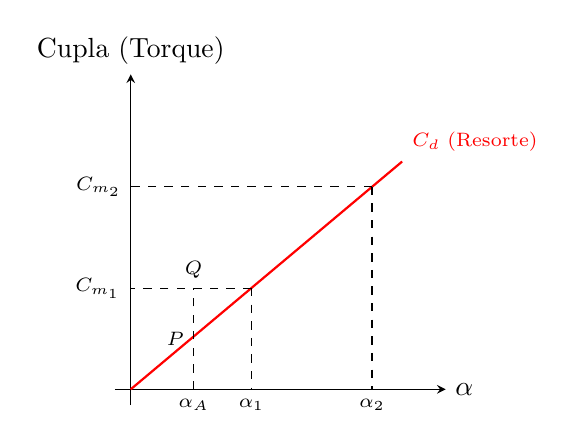
\begin{tikzpicture}[>=stealth]
    % Axis
    \draw[->] (-0.2,0) -- (4,0) node[right] {\(\alpha\)};
    \draw[->] (0,-0.2) -- (0,4) node[above] {Cupla (Torque)};

    % cd curve (Linear Spring)
    \draw[red,thick] (0,0) -- (40:4.5) node[above right] {\scriptsize{\(C_d\) (Resorte)}};

    % intersections to cd (Equilibrium points)
    \draw[dashed] (40:2) -- ++(-1.54,0) node[left] {\scriptsize{\(C_{m_1}\)}};
    \draw[dashed] (40:4) -- ++(-3.06,0) node[left] {\scriptsize{\(C_{m_2}\)}};
    
    % Dropping lines to alpha axis
    \draw[dashed] (40:2) -- ++(0,-1.29) node[below] {\scriptsize{\(\alpha_1\)}};
    \draw[dashed] (40:4) -- ++(0,-2.57) node[below] {\scriptsize{\(\alpha_2\)}};
    
    % Visualizing the forces
    \draw[dashed] (0.8,0) node[below]{\scriptsize{\(\alpha_A\)}} -- node[left]{\scriptsize{\(P\)}} (0.8,1.29) node[above]{\scriptsize{\(Q\)}};
  \end{tikzpicture}
  \caption{Interacción entre Cupla Motora (horizontal) y Directriz (diagonal). El punto de cruce es la lectura final.}
  \label{fig_cuplas_instrumentales}
\end{figure}

\subsection[Cuplas de amortiguamiento]{Cuplas de Amortiguamiento (\(C_a\))}

Esta cupla es necesaria para disipar la energía cinética. Sin ella, la aguja oscilaría mucho tiempo antes de detenerse. Existen tres tipos principales:

\subsubsection{1. Amortiguamiento por Rozamiento Sólido (Indeseable)}
Es el roce entre el eje y los pivotes. \textbf{Es malo} porque introduce un error: la aguja se detiene un poco antes o un poco después del valor real (zona de incertidumbre \(\delta\)).

\subsubsection{2. Amortiguamiento Fluido (Por aire)}
Se usa un aspa moviéndose dentro de una cámara cerrada (como un pistón de aire). Es común en instrumentos de Hierro Móvil.

\subsubsection{3. Amortiguamiento Magnético (Frenado por Corrientes de Foucault)}
Es el más efectivo y elegante. Se basa en la Ley de Lenz: \emph{``El movimiento induce una corriente que se opone a la causa que lo produce''}.

\textbf{¿Cómo funciona paso a paso?} 
\begin{enumerate}
    \item Un disco (o bobina) de aluminio conductor se mueve a velocidad \(v\) dentro de un campo magnético \(B\).
    \item Se induce una fuerza electromotriz (f.e.m.): \( e = B \cdot l \cdot v \).
    \item Como el material es conductor, circula una corriente: \( i = e / R \).
    \item Esta corriente interactúa con el imán creando una fuerza de frenado: \( F = B \cdot l \cdot i \).
\end{enumerate}

Sustituyendo las ecuaciones, obtenemos que el torque de frenado es proporcional a la velocidad angular \(\omega\):
\[ C_a = \left( \frac{B^2 l^2 r^2}{R} \right) \cdot \omega = D \cdot \omega \]
Donde \(D\) es la constante de amortiguamiento. Para que frene bien, necesitamos baja resistencia \(R\) (por eso usamos aluminio) y un campo magnético \(B\) fuerte.

\textbf{Caso especial: Bobina Móvil}
En los instrumentos de bobina móvil, la propia bobina actúa como freno si el circuito externo es de baja resistencia. Además, la bobina suele enrollarse sobre un marco de aluminio. El frenado total es la suma de dos efectos:
\[ D_{\text{total}} = D_{\text{bobina}} + D_{\text{marco aluminio}} \]
\[ D = B^2 l^2 a^2 \left( \underbrace{\frac{N^2}{R}}_{\text{Circuito}} + \underbrace{\frac{S_{Al}}{2\rho(l+a)}}_{\text{Marco de Al}} \right) \]

\subsection{Sistemas de Suspensión}
Para minimizar el error por rozamiento sólido, se utilizan pivotes de alta calidad (piedras preciosas) o, en instrumentos de alta precisión, suspensión por \textbf{cinta tensa}, que elimina totalmente la fricción mecánica al hacer flotar el sistema móvil .
